

\chapter{Results}\label{chap:results}

The table \ref{table:ml_vulnerabilities} shows which types of vulnerabilities (XSS, Path Disclosure, Remote Code Execution, 
and Command Injection) are addressed in the LSTM model.
\begin{table}[H]
 \centering
 \begin{tabular}{lcccc}
 \toprule
 Model & XSS & Path Disclosure & Remote Code Execution & Command Injection \\
 \midrule
 LSTM & \checkmark & \checkmark & \checkmark & \checkmark \\
 CNN & \checkmark & & \checkmark & \\
 MLP & \checkmark & \checkmark & & \\
 GRU & \checkmark & & & \checkmark \\
 \bottomrule
 \end{tabular}
 \caption{Machine Learning Models and Associated Vulnerabilities}
 \label{table:ml_vulnerabilities}
 \end{table}

\subsection{LSTM}

After successfully executing the demonstrat.py script we received the following result for all four vulnerabilities. 
In addition, in this report, we are demonstrating only the first test case due to the report's number of pages.
\begin{itemize}
 \item \textbf{XSS:} Figure \ref{fig:xss_demonstration} shows the result. 
 \begin{figure}
 \centering
 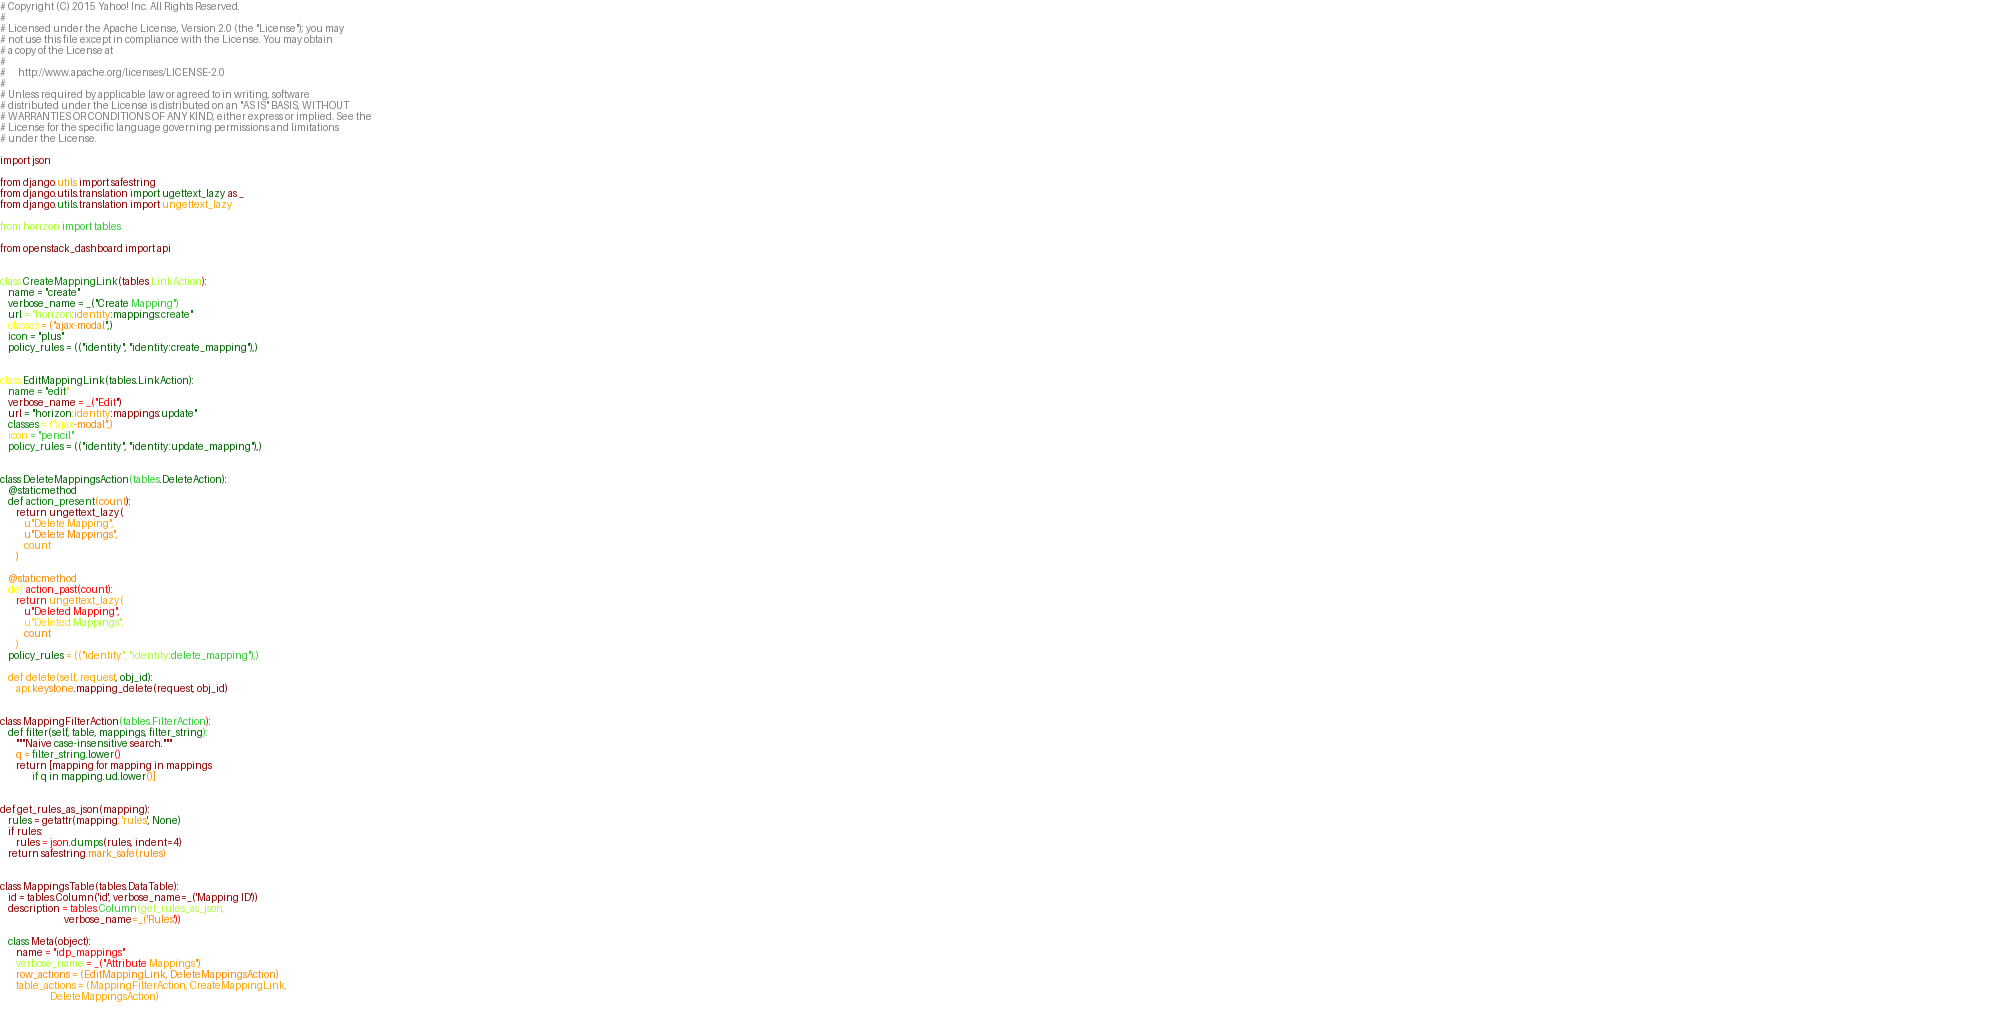
\includegraphics[width=0.5\linewidth]{lstm/demo_xss_1_.png}
 \caption{XSS Demonstration}
 \label{fig:xss_demonstration}
 \end{figure}
 \item \textbf{Command Injection:} Figure \ref{fig:command_injection_demonstration} shows the result.
 \begin{figure}[H]
 \centering
 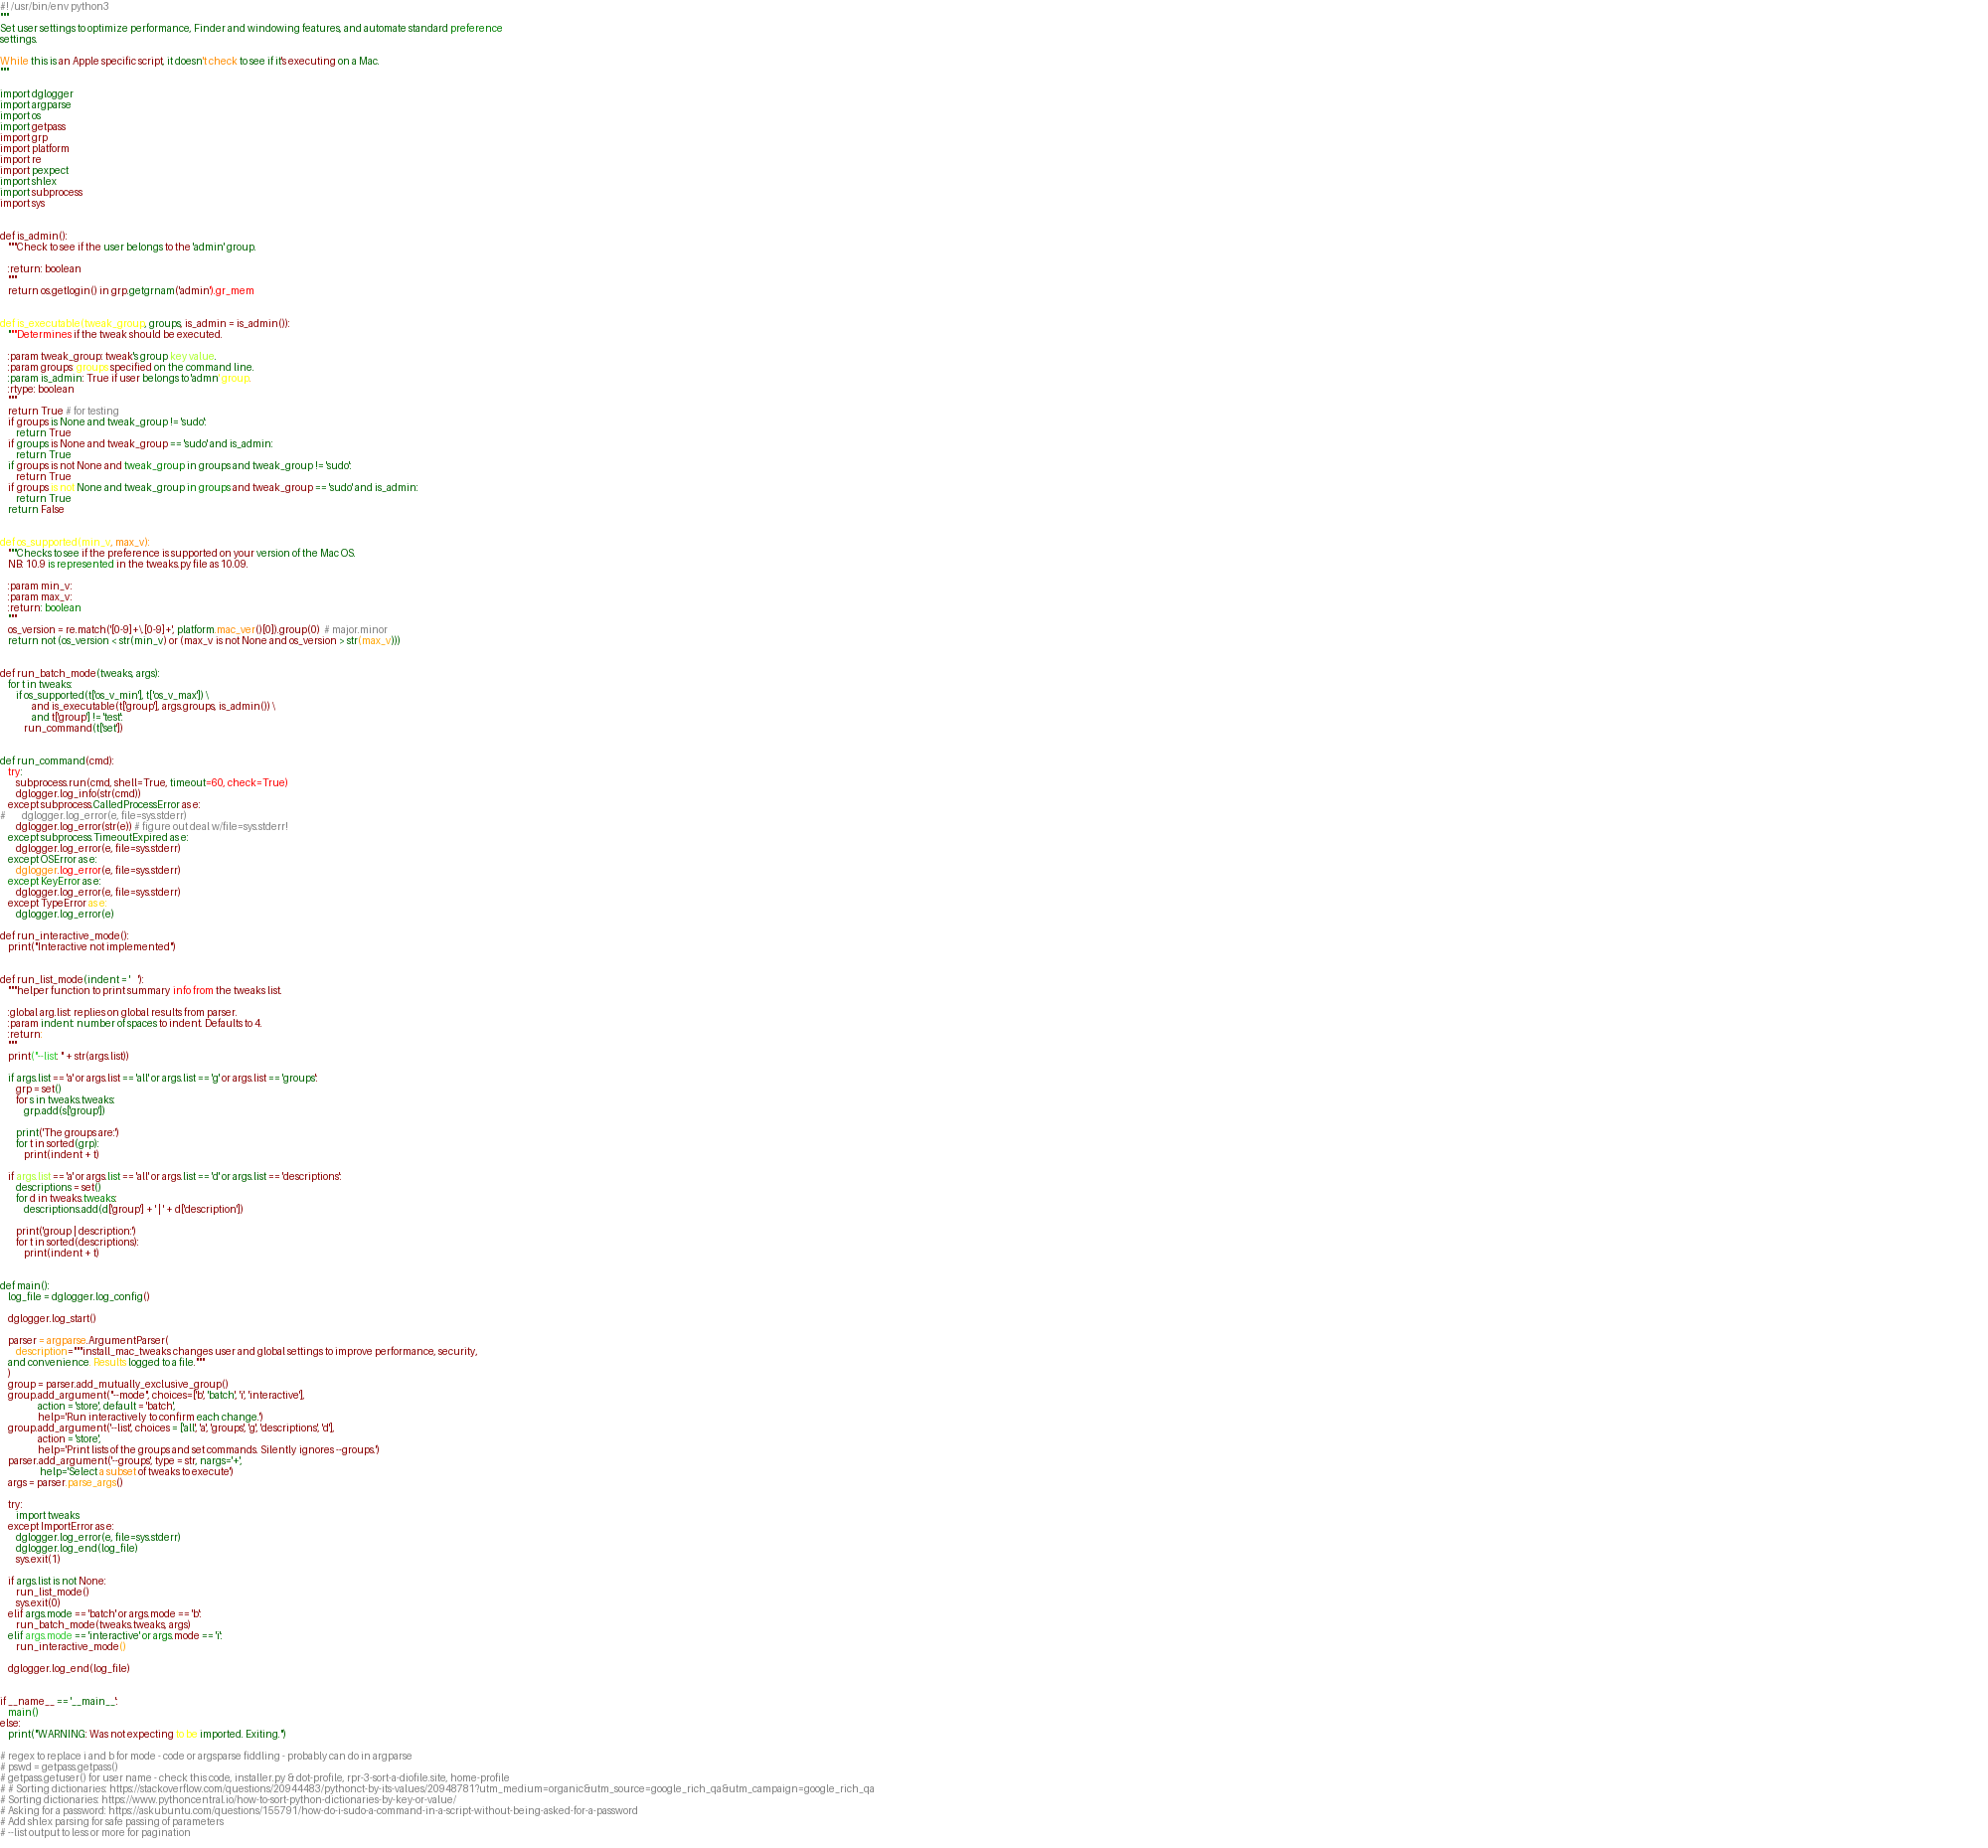
\includegraphics[width=0.5\linewidth]{lstm/demo_command_injection_1_.png}
 \caption{Command Injection Demonstration}
 \label{fig:command_injection_demonstration}
 \end{figure}
 \item \textbf{Remote Code Execution:} Figure \ref{fig:remote_code_execution_demonstration} shows the result.
 \begin{figure}[H]
 \centering
 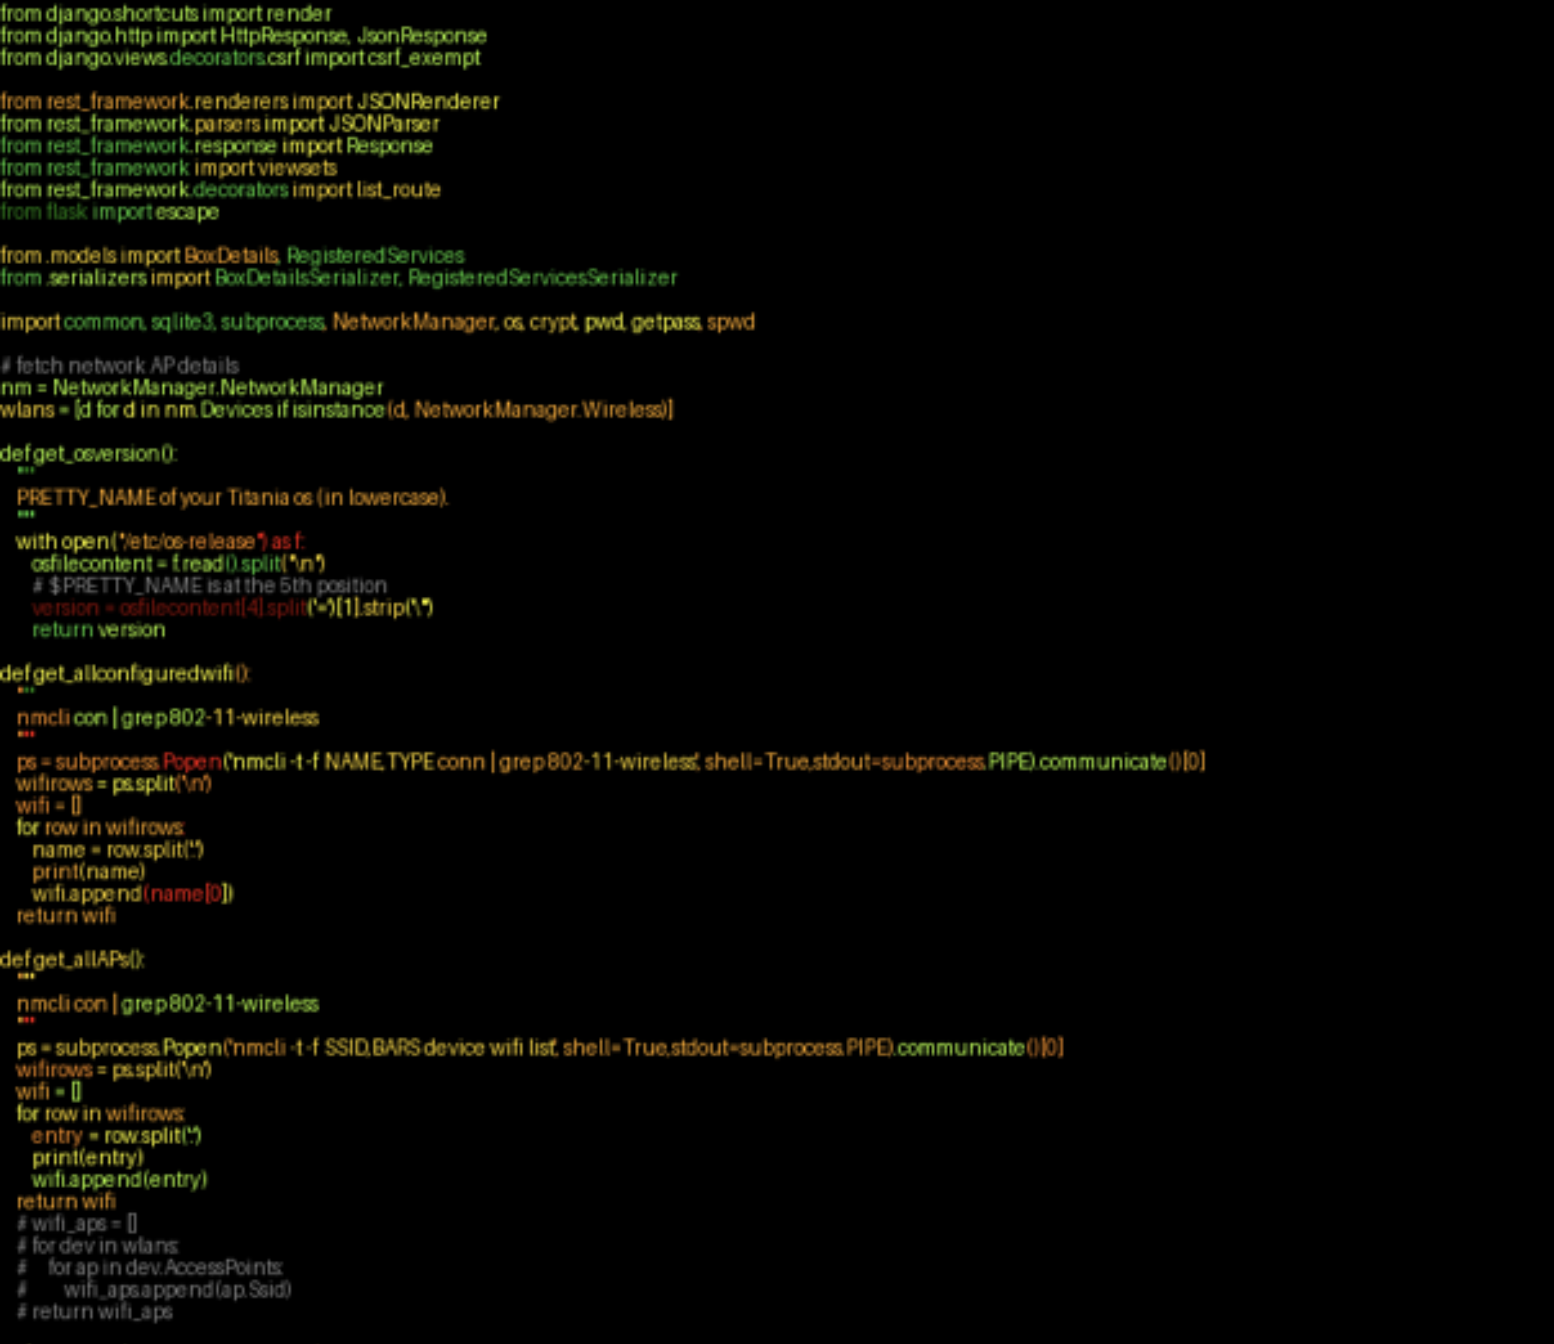
\includegraphics[width=0.5\linewidth]{lstm/demo_remote_code_execution_1_.png}
 \caption{Remote Code Execution Demonstration}
 \label{fig:remote_code_execution_demonstration}
 \end{figure}
 \item \textbf{Path Disclosure:} Figure \ref{fig:path_disclosure_demonstration} shows the result.
 \begin{figure}[H]
 \centering
 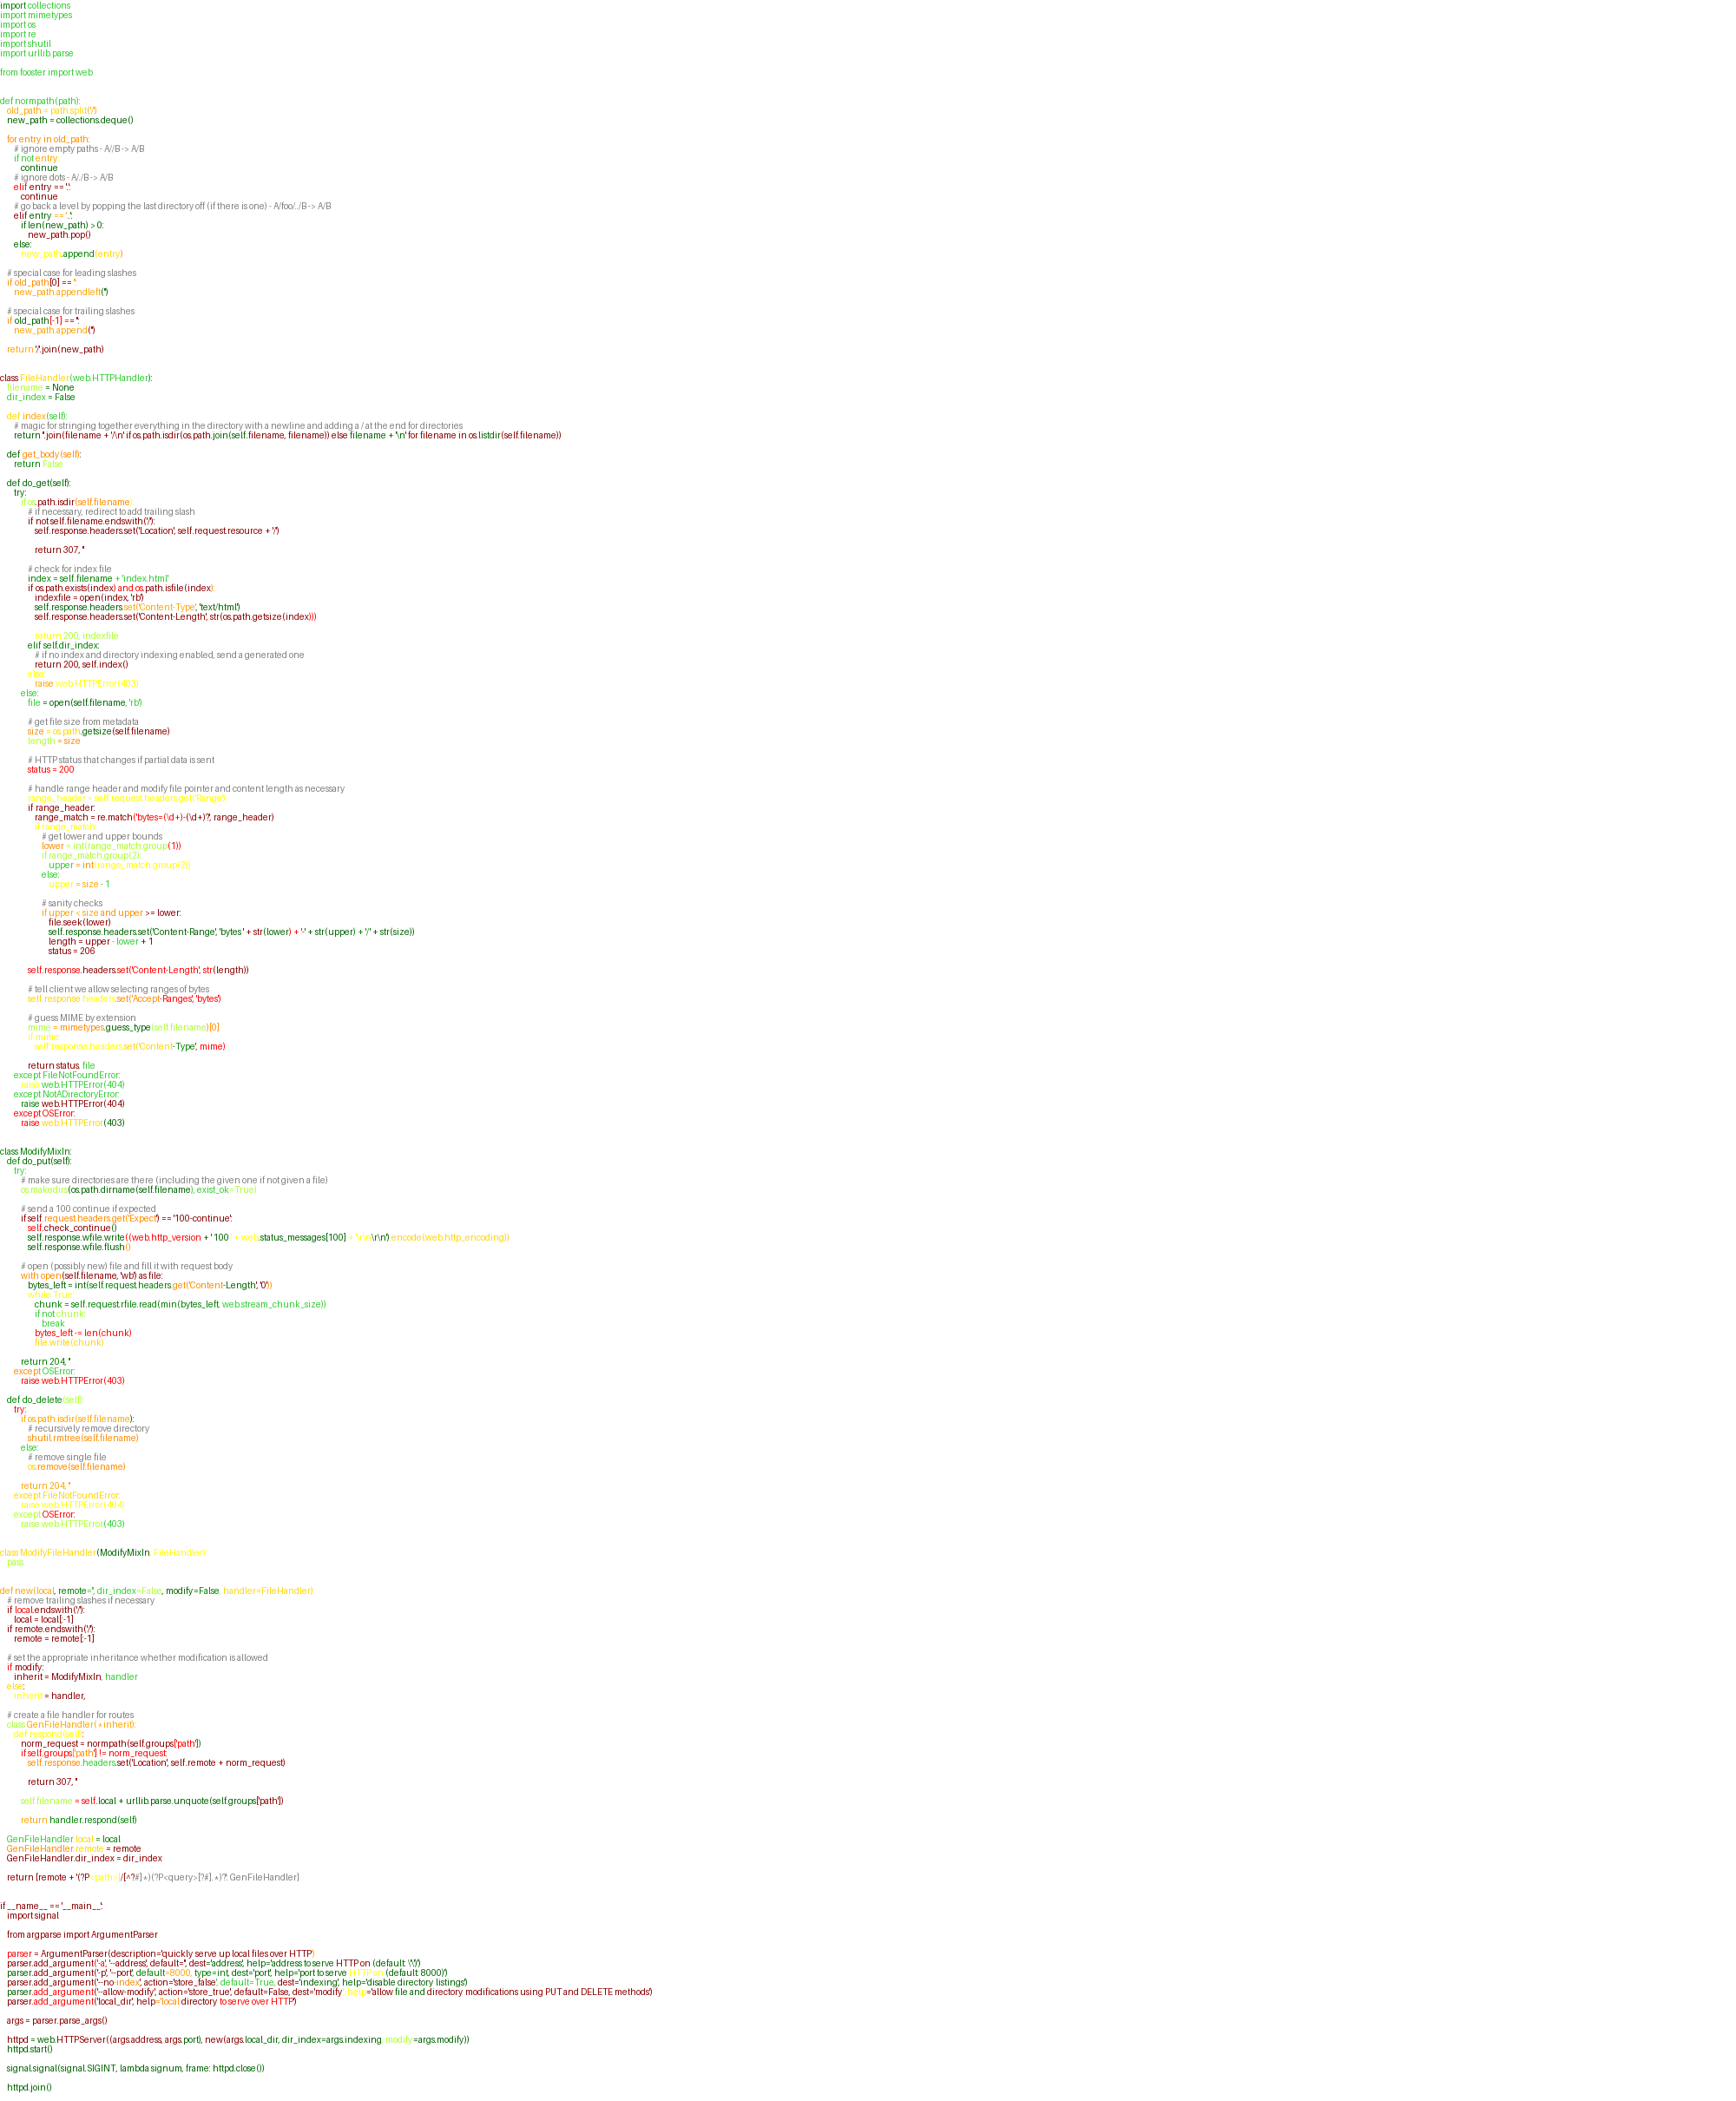
\includegraphics[width=0.5\linewidth]{lstm/demo_path_disclosure_1_.png}
 \caption{Path Disclosure Demonstration}
 \label{fig:path_disclosure_demonstration}
 \end{figure}
\end{itemize}

The table \ref{table:vulnerability_metrics} shows our find out of in LSTM.
\begin{table}[H]
 \centering
 \resizebox{\textwidth}{!}{%
 \begin{tabular}{lrrrrrrr}
 \toprule
 Vulnerability Type & Total Samples &  \% Vulnerable Samples & Absolute Vulnerable Samples & Accuracy & Precision & Recall & F1 Score \\
 \midrule
 General & 8277 & 8.96 & 742 & 0.91035 & 0.91839 & 0.91035 & 0.86763 \\
 Path Disclosure & 19680 & 11.74 & 2311 & 0.88257 & 0.89636 & 0.88257 & 0.82752 \\
 Remote Code Execution & 14412 & 9.08 & 1309 & 0.90917 & 0.91742 & 0.90917 & 0.86592 \\
 Command Injection & 18814 & 12.54 & 2361 & 0.87451 & 0.89026 & 0.87451 & 0.81596 \\
 \bottomrule
 \end{tabular}
 }
 \caption{Vulnerability Statistics and Model Performance Metrics}
 \label{table:vulnerability_metrics}
 \end{table}
 The visualization of the LSTM scores results are shown in chart \ref{fig:model_performance_metrics}.
 \begin{figure}[H]
 \centering
 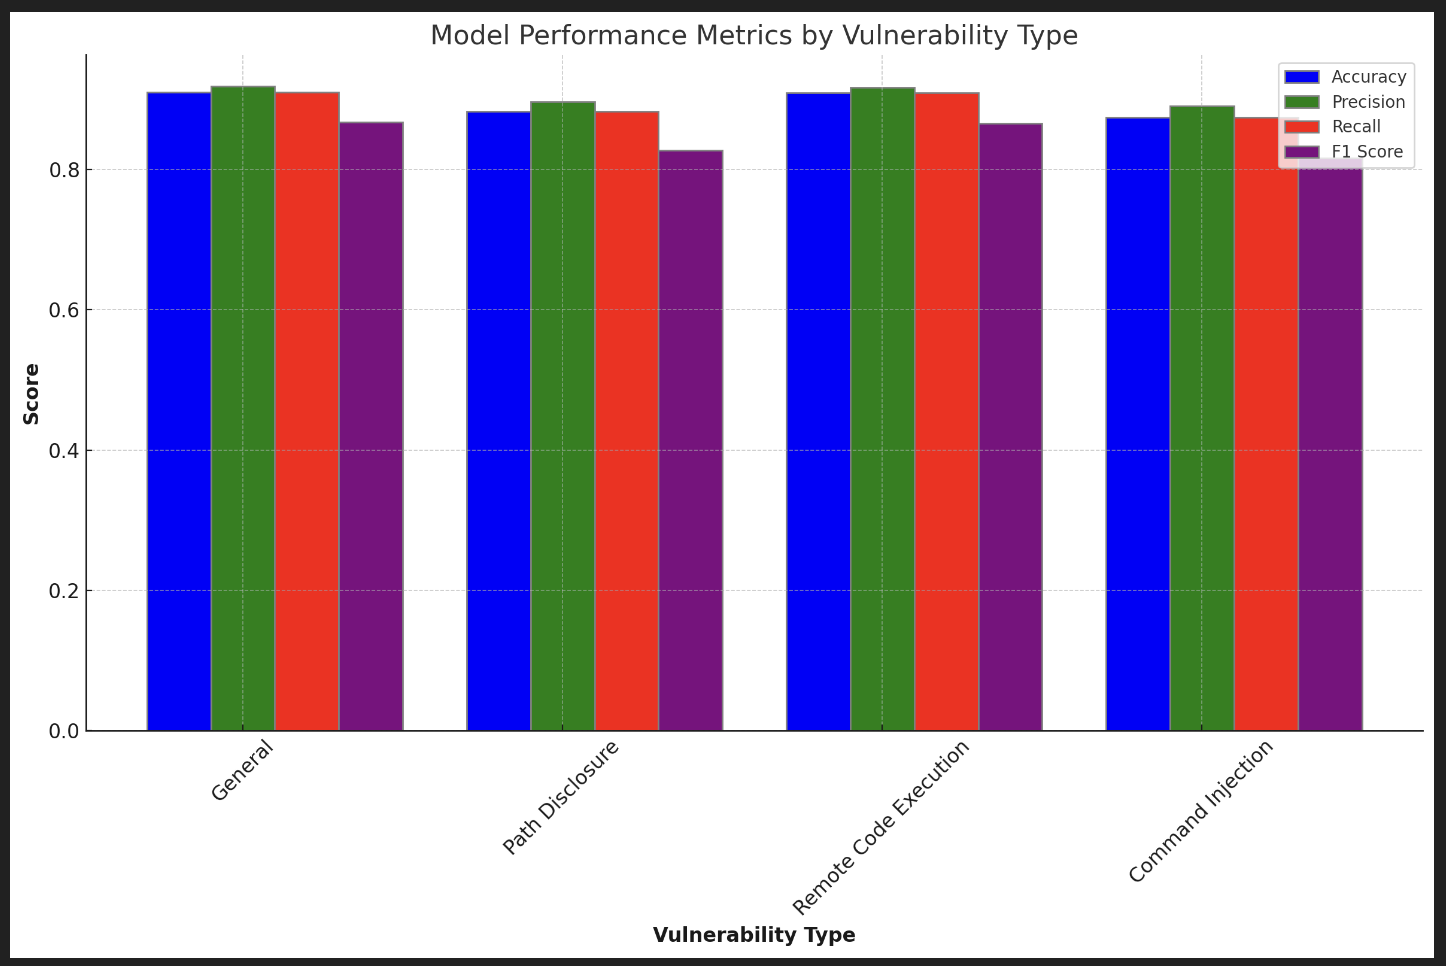
\includegraphics[width=\textwidth]{lstmchart.png}
 \caption{Model Performance Metrics by Vulnerability Type}
 \label{fig:model_performance_metrics}
 \end{figure}
In conclusion, the LSTM model shows good (Accuracy, Precision, Recall, F1Score, Performance consistency), Few false positives, and no false negatives.

% CNN
\subsection{CNN}
The table \ref{table:vulnerability_metrics_xss_rce} shows which types of vulnerabilities (XSS and Remote Code Execution) and their scores in CNN.

\begin{table}[H]
 \centering
 \resizebox{\textwidth}{!}{%
 \begin{tabular}{lrrrrrrr}
 \toprule
 Vulnerability Type & Total Samples &  \% Vulnerable Samples & Absolute Vulnerable Samples & Accuracy & Precision & Recall & F1 Score \\
 \midrule
 XSS & 8277 & 8.34 & 690 & 0.82651 & 0.84052 & 0.82651 & 0.83341 \\
 Remote Code Execution & 14412 & 9.81 & 1414 & 0.16847 & 0.86634 & 0.16847 & 0.15487 \\
 \bottomrule
 \end{tabular}
 }
 \caption{Vulnerability Statistics and Model Performance Metrics for XSS and Remote Code Execution}
 \label{table:vulnerability_metrics_xss_rce}
 \end{table}

Figure \ref{fig:cnnResult} shows the demonstrated result of the CNN model.

\begin{figure}[H]
 \centering
 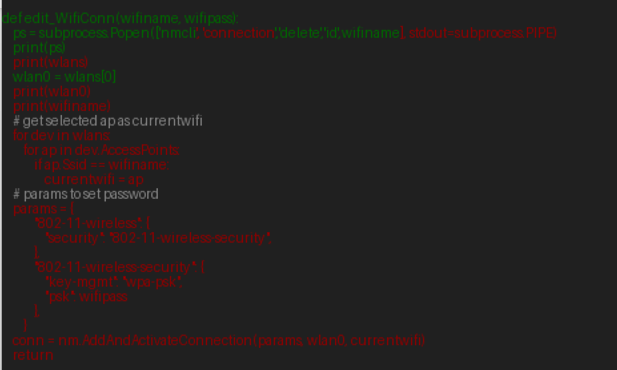
\includegraphics[width=\textwidth]{cnn/cnn1.png}
 \caption{CNN Model Result}
 \label{fig:cnnResult}
\end{figure}

In conclusion, the CNN model shows more false positives and fewer false negatives. Table \ref{table:cnn_model_performance_metrics} demonstrates our conclusion for CNN.

\begin{table}[H]
 \centering
 \resizebox{\textwidth}{!}{%
 \begin{tabular}{lccccccc}
 \toprule
 Vulnerability Type & Accuracy & Precision & Recall & F1 Score \\
 \midrule
 XSS & Good & Good & Good & Good \\
 Remote Code Execution & Poor & Good & Poor & Poor \\
 \bottomrule
 \end{tabular}
 }
 \caption{Model Performance Metrics for Vulnerability Types in CNN}
 \label{table:cnn_model_performance_metrics}
\end{table}

\subsection{MLP}
The table \ref{table:mlpScores} shows which types of vulnerabilities (XSS and Path Disclosure) and their scores in MLP.
\begin{table}[H]
 \centering
 \resizebox{\textwidth}{!}{%
 \begin{tabular}{lrrrrrrr}
 \toprule
 Vulnerability Type & Total Samples &  \% Vulnerable Samples & Absolute Vulnerable Samples & Accuracy & Precision & Recall & F1 Score \\
 \midrule
 XSS & 8277 & 8.88\% & 735 & 89.33\% & 86.47\% & 86.47\% & 87.69\% \\
 Path Disclosure & 19680 & 11.22\% & 2210 & 83.56\% & 71.03\% & 71.03\% & 75.75\% \\
 \bottomrule
 \end{tabular}
 }
 \caption{Vulnerability Statistics and Model Performance Metrics for XSS and Path Disclosure in MLP Modal }
 \label{table:mlpScores}
\end{table}

Figure \ref{fig:mlprdemo} shows the demonstrated result of the MLP model.

\begin{figure}[H]
 \centering
 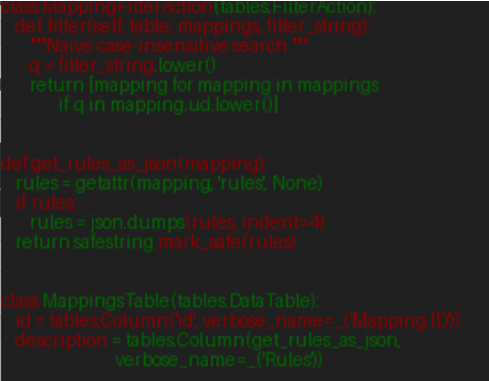
\includegraphics[width=\textwidth]{mlp/mlpresult.png}
 \caption{MLP Model Demonstration}
 \label{fig:mlprdemo}
\end{figure}

In conclusion, the MLP model shows few false positives and few false negatives. Table \ref{table:mlp_model_performance_metrics} demonstrates our conclusion for MLP.

\begin{table}[H]
 \centering
 \resizebox{\textwidth}{!}{%
 \begin{tabular}{lccccccc}
 \toprule
 Vulnerability Type & Accuracy & Precision & Recall & F1 Score \\
 \midrule
 XSS & Good & Good & Good & Good \\
 Path Disclosure & Poor & Good & Poor & Poor \\
 \bottomrule
 \end{tabular}
 }
 \caption{Model Performance Metrics for Vulnerability Types in MLP}
 \label{table:mlp_model_performance_metrics}
\end{table}

\subsection{GRU}
The table \ref{table:mlpScores} shows which types of vulnerabilities (XSS and Command Injection) and their scores in GRU.
\begin{table}[h]
 \centering
 \resizebox{\textwidth}{!}{%
 \begin{tabular}{lccccccc}
 \toprule
 \textbf{Vulnerability Type} & \textbf{Total Samples} & \textbf{\% Vulnerable Samples} & \textbf{Absolute Vulnerable Samples} & \textbf{Accuracy} & \textbf{Precision} & \textbf{Recall} \\ \midrule
 XSS & 8277 & 8.61\% & 713 & 91.39\% & 92.13\% & 91.39\% & 87.27\% \\
 Command Injection & 18814 & 12.73\% & 2396 & 87.26\% & 88.89\% & 87.26\% & 81.33\% \\
 \bottomrule
 \end{tabular}
 }
 \caption{Vulnerability Statistics and Model Performance Metrics for XSS and Command Injection in MLP Modal }
 \label{table:vulnerability_statistics}
\end{table}

Figure \ref{fig:mlprdemo} shows the demonstrated result of the MLP model.
\begin{figure}[H]
 \centering
 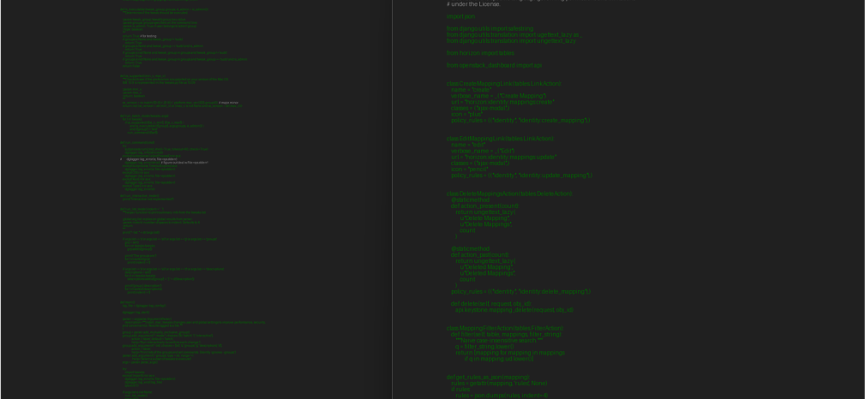
\includegraphics[width=\textwidth]{gru/GRUMDEMO.png}
 \caption{GRU Model Demonstration}
 \label{fig:grudemo}
\end{figure}

We did not conclude GRU because the images were not working. Table \ref{table:mlp_model_performance_metrics} demonstrates our conclusion for GRU.

\begin{table}[H]
 \centering
 \resizebox{\textwidth}{!}{%
 \begin{tabular}{lccccccc}
 \toprule
 Vulnerability Type & Accuracy & Precision & Recall & F1 Score \\
 \midrule
 XSS & Good & Good & Good & Good \\
 Path Disclosure & Poor & Good & Good & Poor \\
 \bottomrule
 \end{tabular}
 }
 \caption{Model Performance Metrics for Vulnerability Types in MLP}
 \label{table:gru_model_performance_metrics}
\end{table}

\subsection{Observations}

After comparing all results we conclude that the LSTM model performance is better than the others. Table \ref{table:all_model_performance_metrics}
\begin{table}[h]
 \centering
 \resizebox{\textwidth}{!} & \textbf{Vulnerable Samples} & \textbf{Accuracy} & \textbf{Precision} & \textbf{Recall} & \textbf{F1 Score} \\
 \midrule
 LSTM & XxSS & & 8277 & 8.96\% & 742 & 0.9104 & 0.9184 & 0.9104 & 0.8676 \\
 & Path Disclosure & & 19680 & 11.74\% & 2311 & 0.8826 & 0.8964 & 0.8826 & 0.8275 \\
 & Remote Code Execution & & 14412 & 9.08\% & 1309 & 0.9092 & 0.9174 & 0.9092 & 0.8659 \\
 MLP & Command Injection & & 18814 & 12.54\% & 2361 & 0.8745 & 0.8903 & 0.8745 & 0.8160 \\
 & XSS & & 8277 & 8.88\% & 735 & 0.8647 & 0.8933 & 0.8647 & 0.8769 \\
 & Path Disclosure & & 19680 & 11.22\% & 2210 & 0.7103 & 0.8356 & 0.7103 & 0.7575 \\
 CNN & XSS & & 8277 & 8.34\% & 690 & 0.8265 & 0.8405 & 0.8265 & 0.8334 \\
 & Remote Code Execution & & 14412 & 9.81\% & 1414 & 0.1685 & 0.8663 & 0.1685 & 0.1549 \\
 GRU & XSS & & 8277 & 8.61\% & 713 & 0.9139 & 0.9213 & 0.9139 & 0.8727 \\
 & Command Injection & & 18814 & 12.73\% & 2396 & 0.8726 & 0.8889 & 0.8726 & 0.8133 \\
 \bottomrule
 \end{tabular}
 }
 \caption{All Models Performance Metrics for Different Vulnerabilities}
 \label{table:all_model_performance_metrics}
\end{table}

The table \ref{table:model_performance_and_observations} shows our observation on average from gathered all results.
\begin{table}[h]
 \centering
 \resizebox{\textwidth}{!}{%
 \begin{tabular}{lccccp{6cm}}
 \toprule
 \textbf{Model} & \textbf{Accuracy (Avg)} & \textbf{Precision (Avg)} & \textbf{Recall (Avg)} & \textbf{F1 Score (Avg)} & \textbf{Observations} \\
 \midrule
 LSTM & 0.8941 & 0.9056 & 0.8941 & 0.8446 & Consistently high accuracy, precision, and recall across all types of vulnerabilities. \\
 MLP & 0.7875 & 0.8645 & 0.7875 & 0.8172 & Strong performance for XSS, but significantly lower for Path Disclosure. \\
 CNN & 0.4975 & 0.8534 & 0.4975 & 0.4942 & Decent performance for XSS but very poor for Remote Code Execution. \\
 GRU & 0.8933 & 0.9051 & 0.8933 & 0.8430 & High performance for XSS and Command Injection, comparable to LSTM. \\
 \bottomrule
 \end{tabular}
 }
 \caption{Performance Metrics and Observations for Different Models}
 \label{table:model_performance_and_observations}
\end{table}